\documentclass{standalone}
\usepackage{tikz}
\usetikzlibrary{patterns, positioning}


\begin{document}
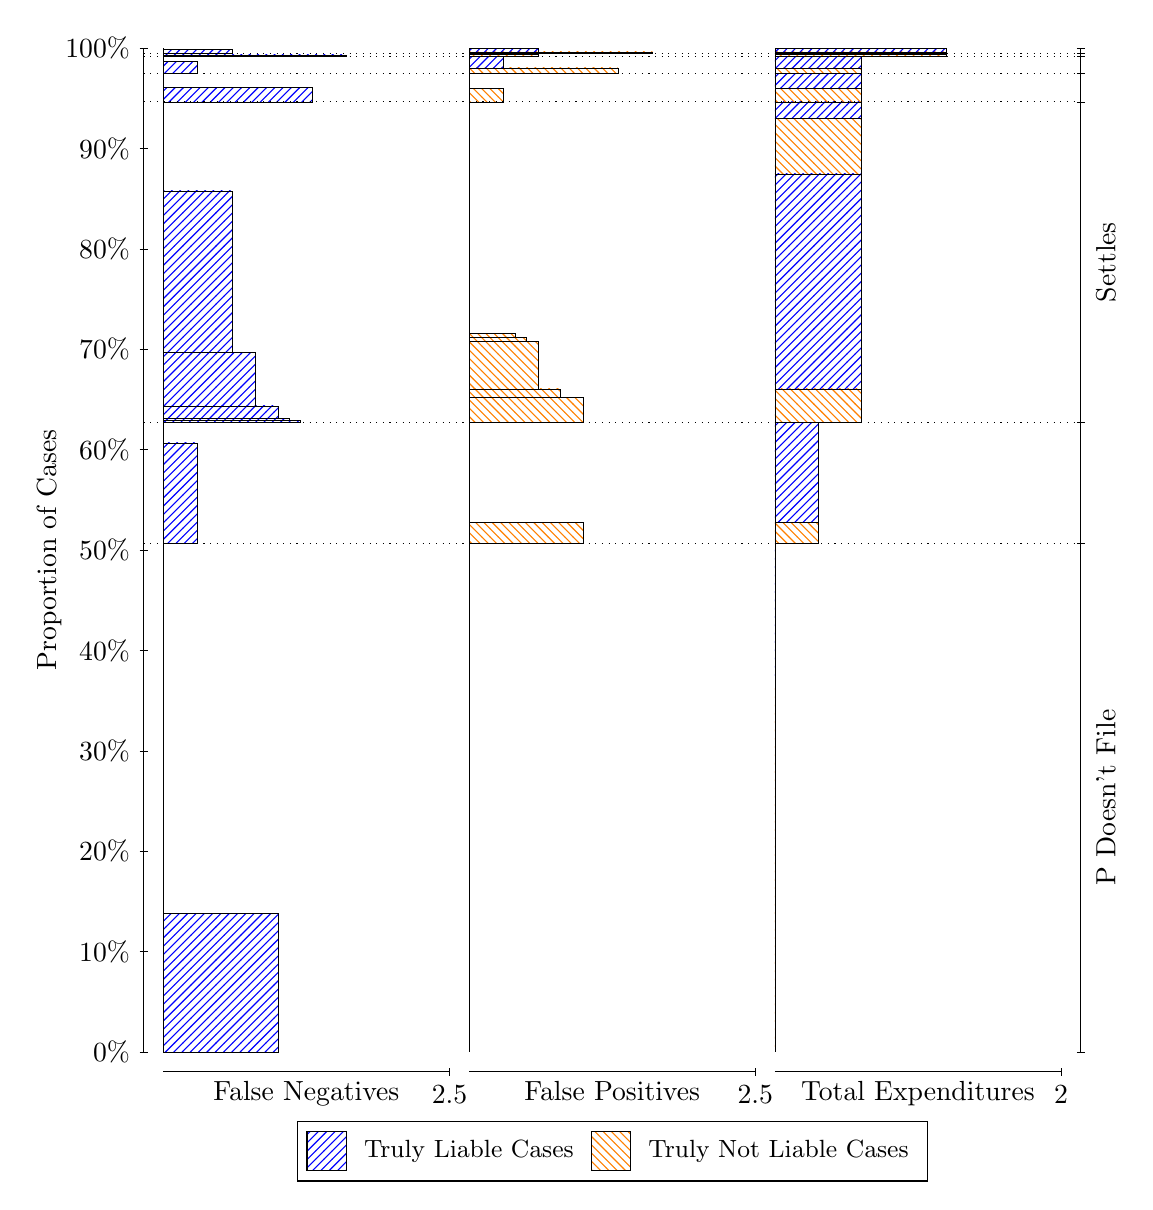
\begin{tikzpicture}
\draw[black, very thin] (1.5,1.75) -- (1.5,14.5);
\node[rotate=90, text=black, anchor=center] at (0.3, 8.125) {Proportion of Cases};
\draw[black, very thin] (1.45,1.75) -- (1.55,1.75);
\node[text=black, anchor=east] at (1.45, 1.75) {0\%};
\draw[black, very thin] (1.45,3.025) -- (1.55,3.025);
\node[text=black, anchor=east] at (1.45, 3.025) {10\%};
\draw[black, very thin] (1.45,4.3) -- (1.55,4.3);
\node[text=black, anchor=east] at (1.45, 4.3) {20\%};
\draw[black, very thin] (1.45,5.575) -- (1.55,5.575);
\node[text=black, anchor=east] at (1.45, 5.575) {30\%};
\draw[black, very thin] (1.45,6.85) -- (1.55,6.85);
\node[text=black, anchor=east] at (1.45, 6.85) {40\%};
\draw[black, very thin] (1.45,8.125) -- (1.55,8.125);
\node[text=black, anchor=east] at (1.45, 8.125) {50\%};
\draw[black, very thin] (1.45,9.4) -- (1.55,9.4);
\node[text=black, anchor=east] at (1.45, 9.4) {60\%};
\draw[black, very thin] (1.45,10.675) -- (1.55,10.675);
\node[text=black, anchor=east] at (1.45, 10.675) {70\%};
\draw[black, very thin] (1.45,11.95) -- (1.55,11.95);
\node[text=black, anchor=east] at (1.45, 11.95) {80\%};
\draw[black, very thin] (1.45,13.225) -- (1.55,13.225);
\node[text=black, anchor=east] at (1.45, 13.225) {90\%};
\draw[black, very thin] (1.45,14.5) -- (1.55,14.5);
\node[text=black, anchor=east] at (1.45, 14.5) {100\%};

\draw[black, very thin] (13.4,1.75) -- (13.4,14.5);
\draw[black, very thin] (13.35,1.75) -- (13.45,1.75);
\node[anchor=west] at (13.35, 1.75) {};
\draw[black, very thin] (13.35,8.2128) -- (13.45,8.2128);
\node[anchor=west] at (13.35, 8.2128) {};
\draw[black, very thin] (13.35,9.7463) -- (13.45,9.7463);
\node[anchor=west] at (13.35, 9.7463) {};
\draw[black, very thin] (13.35,13.816) -- (13.45,13.816);
\node[anchor=west] at (13.35, 13.816) {};
\draw[black, very thin] (13.35,14.178) -- (13.45,14.178);
\node[anchor=west] at (13.35, 14.178) {};
\draw[black, very thin] (13.35,14.398) -- (13.45,14.398);
\node[anchor=west] at (13.35, 14.398) {};
\draw[black, very thin] (13.35,14.436) -- (13.45,14.436);
\node[anchor=west] at (13.35, 14.436) {};
\draw[black, very thin] (13.35,14.5) -- (13.45,14.5);
\node[anchor=west] at (13.35, 14.5) {};

\draw[black, very thin, pattern color=blue, pattern=north east lines] (1.75,1.75) rectangle (3.2033,3.5116);
\draw[black, very thin, pattern color=orange, pattern=north west lines] (1.75,3.5116) rectangle (1.75,8.2128);
\draw[black, very thin, pattern color=blue, pattern=north east lines] (1.75,8.2128) rectangle (2.186,9.4848);
\draw[black, very thin, pattern color=orange, pattern=north west lines] (1.75,9.4848) rectangle (1.75,9.7463);
\draw[black, very thin, pattern color=blue, pattern=north east lines] (1.75,9.7463) rectangle (3.494,9.7664);
\draw[black, very thin, pattern color=blue, pattern=north east lines] (1.75,9.7664) rectangle (3.3487,9.7989);
\draw[black, very thin, pattern color=blue, pattern=north east lines] (1.75,9.7989) rectangle (3.2033,9.9555);
\draw[black, very thin, pattern color=blue, pattern=north east lines] (1.75,9.9555) rectangle (2.9127,10.638);
\draw[black, very thin, pattern color=blue, pattern=north east lines] (1.75,10.638) rectangle (2.622,12.687);
\draw[black, very thin, pattern color=orange, pattern=north west lines] (1.75,12.687) rectangle (1.75,13.816);
\draw[black, very thin, pattern color=blue, pattern=north east lines] (1.75,13.816) rectangle (3.6393,14.002);
\draw[black, very thin, pattern color=orange, pattern=north west lines] (1.75,14.002) rectangle (1.75,14.178);
\draw[black, very thin, pattern color=blue, pattern=north east lines] (1.75,14.178) rectangle (2.186,14.328);
\draw[black, very thin, pattern color=orange, pattern=north west lines] (1.75,14.328) rectangle (1.75,14.398);
\draw[black, very thin, pattern color=blue, pattern=north east lines] (1.75,14.398) rectangle (4.0753,14.414);
\draw[black, very thin, pattern color=orange, pattern=north west lines] (1.75,14.414) rectangle (1.75,14.436);
\draw[black, very thin, pattern color=blue, pattern=north east lines] (1.75,14.436) rectangle (2.622,14.484);
\draw[black, very thin, pattern color=orange, pattern=north west lines] (1.75,14.484) rectangle (1.75,14.5);
\draw[black, very thin, pattern color=orange, pattern=north west lines] (5.6333,1.75) rectangle (5.6333,6.4512);
\draw[black, very thin, pattern color=blue, pattern=north east lines] (5.6333,6.4512) rectangle (5.6333,8.2128);
\draw[black, very thin, pattern color=orange, pattern=north west lines] (5.6333,8.2128) rectangle (7.0867,8.4743);
\draw[black, very thin, pattern color=blue, pattern=north east lines] (5.6333,8.4743) rectangle (5.6333,9.7463);
\draw[black, very thin, pattern color=orange, pattern=north west lines] (5.6333,9.7463) rectangle (7.0867,10.065);
\draw[black, very thin, pattern color=orange, pattern=north west lines] (5.6333,10.065) rectangle (6.796,10.171);
\draw[black, very thin, pattern color=orange, pattern=north west lines] (5.6333,10.171) rectangle (6.5053,10.77);
\draw[black, very thin, pattern color=orange, pattern=north west lines] (5.6333,10.77) rectangle (6.36,10.829);
\draw[black, very thin, pattern color=orange, pattern=north west lines] (5.6333,10.829) rectangle (6.2147,10.875);
\draw[black, very thin, pattern color=blue, pattern=north east lines] (5.6333,10.875) rectangle (5.6333,13.816);
\draw[black, very thin, pattern color=orange, pattern=north west lines] (5.6333,13.816) rectangle (6.0693,13.992);
\draw[black, very thin, pattern color=blue, pattern=north east lines] (5.6333,13.992) rectangle (5.6333,14.178);
\draw[black, very thin, pattern color=orange, pattern=north west lines] (5.6333,14.178) rectangle (7.5227,14.248);
\draw[black, very thin, pattern color=blue, pattern=north east lines] (5.6333,14.248) rectangle (6.0693,14.398);
\draw[black, very thin, pattern color=orange, pattern=north west lines] (5.6333,14.398) rectangle (6.5053,14.42);
\draw[black, very thin, pattern color=blue, pattern=north east lines] (5.6333,14.42) rectangle (5.6333,14.436);
\draw[black, very thin, pattern color=orange, pattern=north west lines] (5.6333,14.436) rectangle (7.9587,14.451);
\draw[black, very thin, pattern color=blue, pattern=north east lines] (5.6333,14.451) rectangle (6.5053,14.5);
\draw[black, very thin, pattern color=orange, pattern=north west lines] (9.5167,1.75) rectangle (9.5167,6.4512);
\draw[black, very thin, pattern color=blue, pattern=north east lines] (9.5167,6.4512) rectangle (9.5167,8.2128);
\draw[black, very thin, pattern color=orange, pattern=north west lines] (9.5167,8.2128) rectangle (10.062,8.4743);
\draw[black, very thin, pattern color=blue, pattern=north east lines] (9.5167,8.4743) rectangle (10.062,9.7463);
\draw[black, very thin, pattern color=orange, pattern=north west lines] (9.5167,9.7463) rectangle (10.607,10.171);
\draw[black, very thin, pattern color=blue, pattern=north east lines] (9.5167,10.171) rectangle (10.607,12.903);
\draw[black, very thin, pattern color=orange, pattern=north west lines] (9.5167,12.903) rectangle (10.607,13.607);
\draw[black, very thin, pattern color=blue, pattern=north east lines] (9.5167,13.607) rectangle (10.607,13.816);
\draw[black, very thin, pattern color=orange, pattern=north west lines] (9.5167,13.816) rectangle (10.607,13.992);
\draw[black, very thin, pattern color=blue, pattern=north east lines] (9.5167,13.992) rectangle (10.607,14.178);
\draw[black, very thin, pattern color=orange, pattern=north west lines] (9.5167,14.178) rectangle (10.607,14.248);
\draw[black, very thin, pattern color=blue, pattern=north east lines] (9.5167,14.248) rectangle (10.607,14.398);
\draw[black, very thin, pattern color=orange, pattern=north west lines] (9.5167,14.398) rectangle (11.697,14.42);
\draw[black, very thin, pattern color=blue, pattern=north east lines] (9.5167,14.42) rectangle (11.697,14.436);
\draw[black, very thin, pattern color=orange, pattern=north west lines] (9.5167,14.436) rectangle (11.697,14.451);
\draw[black, very thin, pattern color=blue, pattern=north east lines] (9.5167,14.451) rectangle (11.697,14.5);
\draw[black, dotted] (1.5,8.2128) -- (13.4,8.2128);
\draw[black, dotted] (1.5,9.7463) -- (13.4,9.7463);
\draw[black, dotted] (1.5,13.816) -- (13.4,13.816);
\draw[black, dotted] (1.5,14.178) -- (13.4,14.178);
\draw[black, dotted] (1.5,14.398) -- (13.4,14.398);
\draw[black, dotted] (1.5,14.436) -- (13.4,14.436);
\draw[black, very thin] (1.75,1.5) -- (5.3833,1.5);
\node[text=black, anchor=north] at (3.5667, 1.5) {False Negatives};
\draw[black, very thin] (5.3833,1.45) -- (5.3833,1.55);
\node[text=black, anchor=north] at (5.3833, 1.45) {2.5};

\draw[black, very thin] (5.6333,1.5) -- (9.2667,1.5);
\node[text=black, anchor=north] at (7.45, 1.5) {False Positives};
\draw[black, very thin] (9.2667,1.45) -- (9.2667,1.55);
\node[text=black, anchor=north] at (9.2667, 1.45) {2.5};

\draw[black, very thin] (9.5167,1.5) -- (13.15,1.5);
\node[text=black, anchor=north] at (11.333, 1.5) {Total Expenditures};
\draw[black, very thin] (13.15,1.45) -- (13.15,1.55);
\node[text=black, anchor=north] at (13.15, 1.45) {2};

\node[text=black, centered, rotate=90] at (13.72, 4.9814) {P Doesn't File};

\node[text=black, centered, rotate=90] at (13.72, 11.781) {Settles};





\draw (7.449999999999999,1.5) node[draw=none] (baseCoordinate) {};
\begin{scope}[align=center]
        \matrix[scale=0.5, draw=black, below=0.5cm of baseCoordinate, nodes={draw}, column sep=0.1cm]{
            \node[rectangle, draw, minimum width=0.5cm, minimum height=0.5cm, pattern color=blue, pattern=north east lines] {}; &
            \node[draw=none, font=\small, text=black] (B) {Truly Liable Cases}; &
            \node[rectangle, draw, minimum width=0.5cm, minimum height=0.5cm, pattern color=orange, pattern=north west lines] {}; &
            \node[draw=none, font=\small, text=black] (B) {Truly Not Liable Cases}; \\
            };
\end{scope}

\end{tikzpicture}
\end{document}